\documentclass{beamer}


% zum ausdrucken
% \documentclass[handout]{beamer}

% Schneller Kompilieren 
% \documentclass[draft]{beamer}


\usepackage{lmodern,dsfont}
\usepackage{rotating}
\usepackage{geometry}
\usepackage{mathtools}
\usepackage{listings}
\usepackage{wrapfig}
\usepackage{lscape}
\usepackage{beamerthemesplit}
\usepackage[ngerman]{babel}
\usepackage[T1]{fontenc}
\usepackage[utf8]{inputenc}
%\usepackage{uniinput}
\usepackage{multirow}
\usepackage{textcomp}
\usetheme{Darmstadt}
%Gute: Warsaw, Berlin, CambridgeUS, Copenhagen,Darmstadt, Ilmenau, Frankfurt
% nicht so Gute:
%, AnnArbor, Antibes,Bergen, Berkeley, Boadilla, boxes,default,Dresden, Szeged, Singapore, Rochester
%Pittsburgh, PaloAlto, Montpellier, Marburg, Malmoe, Madrid, Luebeck,JuanLesPins, Hannover, Goettingen

\usecolortheme{orchid}
% gute dolphin, orchid, rose
%Andere Frabgebeungen: albatross,beaver, beetle, crane, default, dove, fly, lily, seagull, seahorse, sidebartab, wolverine

%\useinnertheme{rounded}
%Andere: ,inmargin circles, rectangles

%\useoutertheme{tree}
%Andrer: infolines ,miniframes, shadow, smoothbars, smoothtree, split,tree

\setbeamercovered{transparent}

\beamertemplatenavigationsymbolsempty
\setbeamertemplate{footline}[frame number]


%Für Quellcode
\usepackage{listings}
\usepackage{color}
\usepackage{textcomp}

\lstset{language=Java,
   basicstyle=\tiny,
   keywordstyle=\color{blue!80!black!100},
   identifierstyle=,
   commentstyle=\color{green!50!black!100},
   stringstyle=\ttfamily,
   breaklines=true,
   numbers=left,
   numberstyle=\small,
   frame=single,
   backgroundcolor=\color{blue!3}
} 

\title{Solert - Concept}
\author{Timon Back, Lars Oetermann}
\date[]{}
\begin{document}
\frame{\titlepage}
%\frame{\tableofcontents}

\section{Goal}
\frame
{
\frametitle{What our Webpage should provide}
  \begin{itemize}
   \item Insert your location (city, zip, address)
   \item Present two graphs:
      \begin{itemize} 
	\item with a detailed sun forecast of the next 3 hours
	\item with a rough sun forecast of the next 24 hours
	\end{itemize}
    \item Optional:
      \begin{itemize}
       \item User management to save favorite locations
       \item Location selection via a 2D map of the Netherlands
       \item Embedding the sun-map-view from buienradar.nl
      \end{itemize}

  \end{itemize}

}

\begin{frame}
 
 \frametitle{Paper Prototype}
 \begin{center}
   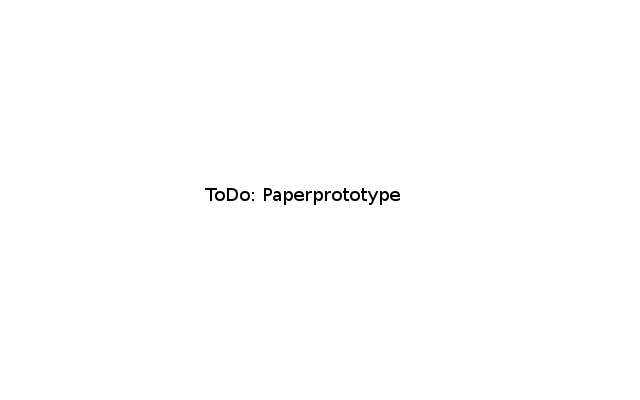
\includegraphics[width=0.9\textwidth]{paperprototype.png}
 \end{center}

\end{frame}


\section{Services}
\frame
{
\frametitle{Services we use and provide}\begin{columns}[c]  
   \column{.5\textwidth}
    \begin{block}{Sunforecast Data Crawler}
	\begin{description}
	  \item[Provide:] sun forecast data
	  \item[Using:] buienradar.nl
	  \item[Our task:] fetch data from buienradar.nl and store in our database
	 \end{description}
     \end{block}
     \begin{block}{Graph Plotting}
	\begin{description} 
	  \item[Provide:] line or bar graph
	  \item[Using:] ChartJS.org
	  \item[Our task:] plotting a graph based on forecast data
	\end{description}
     \end{block}
   \column{.5\textwidth}
   \begin{block}{Location conversion}
     \begin{description}  
	\item[Provide:] latitude/longitude
	\item[Using:] googleapis.com
	\item[Our task:] convert the location (city, zip, address) into latitude/longitude
     \end{description}
   \end{block}
 \end{columns}
}


\begin{frame}
 
 \frametitle{Service Diagram}
 \begin{center}
   \includegraphics[width=0.9\textwidth]{service-diagram.png}
 \end{center}

\end{frame}

% For Code use \begin{lstlisting}   \end{lstlisting}
 
 
      
\end{document}